\documentclass{dcpresentation}

% Presentation info
\title{Introduction to Kubernetes}
\author{}
\newcommand{\authorEmail}{}
\institute{SciLifeLab Data Centre}
\date{}

\usepackage{listings}

\usepackage{xcolor}

\usepackage{enumerate}

\usepackage{tikz}
\usetikzlibrary{calc,fadings}
\tikzfading[name=fade l,left color=transparent!100,right color=transparent!0]
\tikzfading[name=fade r,right color=transparent!100,left color=transparent!0]
\tikzfading[name=fade d,bottom color=transparent!100,top color=transparent!0]
\tikzfading[name=fade u,top color=transparent!100,bottom color=transparent!0]

% this "frames" a rectangle node
\newcommand\framenode[2][10pt]{
    \fill[white,path fading=fade u] (#2.south west) rectangle ($(#2.south east)+(0, #1)$);
    \fill[white,path fading=fade d] (#2.north west) rectangle ($(#2.north east)+(0,-#1)$);
    \fill[white,path fading=fade l] (#2.south east) rectangle ($(#2.north east)+(-#1,0)$);
    \fill[white,path fading=fade r] (#2.south west) rectangle ($(#2.north west)+( #1,0)$);
}

\definecolor{commentsColor}{rgb}{0.497495, 0.497587, 0.497464}
\definecolor{keywordsColor}{rgb}{0.000000, 0.000000, 0.635294}
\definecolor{stringColor}{rgb}{0.558215, 0.000000, 0.135316}
 
\lstset{ %
  backgroundcolor=\color{white},   % choose the background color; you must add \usepackage{color} or \usepackage{xcolor}
  basicstyle=\footnotesize,        % the size of the fonts that are used for the code
  breakatwhitespace=false,         % sets if automatic breaks should only happen at whitespace
  breaklines=true,                 % sets automatic line breaking
  captionpos=b,                    % sets the caption-position to bottom
  commentstyle=\color{commentsColor}\textit,    % comment style
  deletekeywords={...},            % if you want to delete keywords from the given language
  escapeinside={\%*}{*)},          % if you want to add LaTeX within your code
  extendedchars=true,              % lets you use non-ASCII characters; for 8-bits encodings only, does not work with UTF-8
  keepspaces=true,                 % keeps spaces in text, useful for keeping indentation of code (possibly needs columns=flexible)
  keywordstyle=\color{keywordsColor}\bfseries,       % keyword style
  language=Python,                 % the language of the code (can be overrided per snippet)
  otherkeywords={*,...},           % if you want to add more keywords to the set
  rulecolor=\color{black},         % if not set, the frame-color may be changed on line-breaks within not-black text (e.g. comments (green here))
  showspaces=false,                % show spaces everywhere adding particular underscores; it overrides 'showstringspaces'
  showstringspaces=false,          % underline spaces within strings only
  showtabs=false,                  % show tabs within strings adding particular underscores
  stepnumber=1,                    % the step between two line-numbers. If it's 1, each line will be numbered
  stringstyle=\color{stringColor}, % string literal style
  tabsize=2,                      % sets default tabsize to 2 spaces
  title=\lstname,                  % show the filename of files included with \lstinputlisting; also try caption instead of title
  columns=fixed                    % Using fixed column width (for e.g. nice alignment)
}



\begin{document}
 \begin{frame}
  \maketitle
 \end{frame}

  % put logo in upper right corner to ape the official template
 \AddToShipoutPictureFG{
  \AtPageUpperRight{{
\includegraphics[width=0.6cm,keepaspectratio]{img/scilifelab-symbol.pdf}}}
 }%
 
 \begin{frame}{Containers}
  \begin{itemize}
   \item ``Environment'' in a running operating system
   \item Not a virtual machine
   \item Kernel namespaces
   \begin{itemize}
    \item Processes
    \item Network interfaces
    \item Filesystem mount points
    \item ...
   \end{itemize}
  \end{itemize}
 \end{frame}
 
 \begin{frame}[fragile]{Dockerfile}
 \scriptsize
  \begin{verbatim}
FROM node:latest as build

RUN yarn global add @quasar/cli
COPY ./frontend/package.json /package.json
WORKDIR /
RUN yarn install
COPY ./frontend /code
RUN mv /node_modules /code/
WORKDIR /code
RUN quasar build


FROM nginx:alpine

COPY --from=build /code/dist/spa/ /usr/share/nginx/html/
COPY ./k8s/nginx.conf /etc/nginx/nginx.conf

EXPOSE 80
  \end{verbatim}
 \end{frame}


 \begin{frame}{Kubernetes}
  \begin{itemize}
   \item Container orchestration
   \item Originates from Google
   \item Kubernetes $\rightarrow$ K + 8 letters + s $\rightarrow$ k8s (``Kates'')
  \end{itemize}
 \end{frame}
 
 \begin{frame}{Basics}
  \begin{itemize}
   \item \texttt{kubectl}
   \begin{itemize}
    \item \texttt{kubectl apply -f ...}
    \item \texttt{kubectl delete -f ...}
    \item \texttt{kubectl get ...}
    \item \texttt{kubectl describe ...}
   \end{itemize}
   \item ``Death by \texttt{YAML}''
  \end{itemize}
 \end{frame}
  % Demo:
  % kubectl get (pods)
  % kubectl describe (pods)
  % kubectl apply
  % kubectl delete
  
 \begin{frame}[fragile]{Example}
  \small
  \begin{verbatim}
apiVersion: v1
kind: Pod
metadata:
  name: menu-backend
spec:
  containers:
  - name: menu-backend
    image: scilifelabdatacentre/menu-backend:latest
    ports:
    - containerPort: 8000
  \end{verbatim}
 \end{frame}
 
  \begin{frame}[fragile]{Example}
  \tiny
  \begin{columns}
   \column{0.4\textwidth}
\begin{verbatim}
apiVersion: apps/v1
kind: Deployment
metadata:
  name: dsw-client
  labels:
    name: dsw-client
    type: prod
  namespace: dc-dsw
spec:
  selector:
    matchLabels:
      name: dsw-client
      type: prod
  replicas: 1
  template:
    metadata:
      labels:
        name: dsw-client
        type: prod
        version: 2.5.0
    spec:
      containers:
      - name: dsw-client
        image: dsw/wizard-client:2.5.0
        resources:
          limits:
            cpu: 600m
            memory: 200Mi
          requests:
            cpu: 200m
            memory: 40Mi
    \end{verbatim}
     \column{0.6\textwidth}
  \begin{verbatim}
        ports:
          - containerPort: 80
        readinessProbe:
          httpGet:
            path: /
            scheme: HTTP
            port: 80
        volumeMounts:
          - name: client-conf
            mountPath: /src/scss/_variables.scss
            subPath: _variables.scss
          - name: client-conf
            mountPath: /src/scss/_overrides.scss
            subPath: _overrides.scss
          - name: custom-assets
            mountPath: /usr/share/nginx/html/assets
        env:
          - name: API_URL
            valueFrom:
              configMapKeyRef:
                name: prod-client
                key: API_URL
      volumes:
        - name: client-conf
          configMap:
            name: prod-client
        - name: custom-assets
          configMap:
            name: custom-assets

  \end{verbatim}
    \end{columns}

 \end{frame}
 
 \begin{frame}{Namespace}
  \begin{itemize}
   \item Internal grouping
   \item DNS
   \begin{itemize}
    \item \texttt{<service>.<namespace>.svc.cluster.local}
   \end{itemize}
   \item Access/resource control
  \end{itemize}
 \end{frame}
 
  \begin{frame}{Pods}
  \centering
  
\includegraphics[width=0.8\textwidth]{img/arch-p.pdf}
 \end{frame}
 
 \begin{frame}{Pods}
  \begin{itemize}
   \item ``Basic unit''
   \item One or more containers in each pod
   \item A deleted pod won't restart
  \end{itemize}
 \end{frame}
 % Demo:
 % - start pod
 % - show it's running
 % - delete pod
 % - show it's gone
 
  % Demo:
 % - start deployment
 % - show it's running kubectl get pods/rs/deploy
 % - delete pod
 % - show it's replaced
 % - deploy new version
 % - show gradual change kubectl get pods rs deploy
 % - delete deployment
 % - show it's gone
 
 \begin{frame}{Volumes}
  \begin{itemize}
   \item Persistent storage
   \item \texttt{PersistentVolume}
   \begin{itemize}
    \item Storage, e.g. a folder on a hd or nfs
    \item Global
   \end{itemize}
   \item \texttt{StorageClass}
   \begin{itemize}
    \item Storage pool
    \item Global
   \end{itemize}
   \item \texttt{PersistentVolumeClaim}
   \begin{itemize}
    \item The ``claim'' for storage used by the pod.
    \item Namespaced
   \end{itemize}
  \end{itemize}
 \end{frame}

 \begin{frame}{Configuration Variables and Files}
   \begin{itemize}
    \item \texttt{env:}
    \item ConfigMap
    \item Secret
    \begin{itemize}
     \item Not encrypted
     \item Base64
    \end{itemize}
    \item Use cases:
    \begin{itemize}
     \item Environment variables
     \item Arguments
     \item Files
    \end{itemize}
   \end{itemize}
 
 \end{frame}
 
 \begin{frame}{Services}
  \centering
  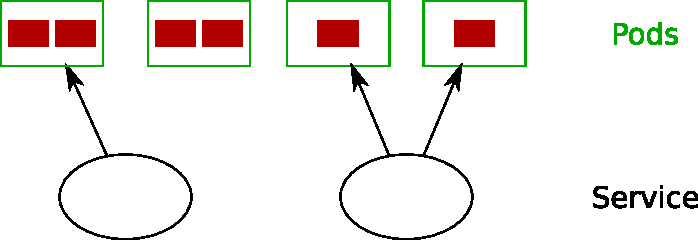
\includegraphics[width=0.8\textwidth]{img/arch-ps.pdf}
 \end{frame}
 
 \begin{frame}{Services}
  \begin{itemize}
   \item Allow easy access (``DNS'') to groups of pods
   \item Selecting pods using labels
   \item Can be used to expose pods to external access
   \item Load balancing
  \end{itemize}
 \end{frame}

 % Demo:
 % - start service
 % - describe - show that pods are found

 \begin{frame}{Ingress}
  \centering
  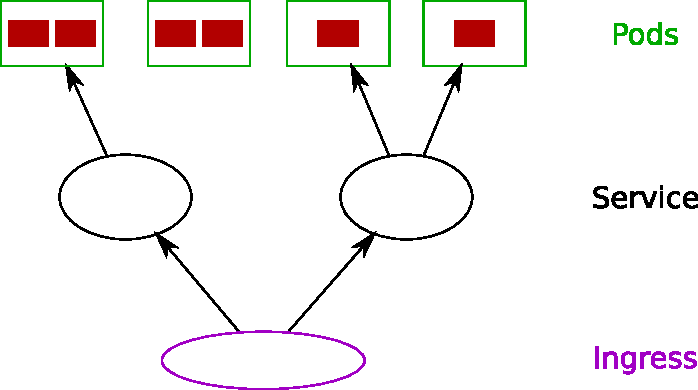
\includegraphics[width=0.8\textwidth]{img/arch-psi.pdf}
 \end{frame}
 
 \begin{frame}{Ingress}
  \begin{itemize}
   \item Http(s) access to containers
   \item Certmanager
   \begin{itemize}
    \item Certification management
    \item Integration with Let's Encrypt
   \end{itemize}
   \item Interface
   \begin{itemize}
    \item No official implementation
   \end{itemize}
   \item Multiple available
   \begin{itemize}
    \item Nginx
    \item GCE
    \item AWS ALB Ingress Controller
    \item Traefik
    \item ...
   \end{itemize}
  \end{itemize}
 \end{frame}
 
 % Demo:
 % - start ingress
 % - describe - show that service -> pod is found
 % - access from browser
 
 \begin{frame}{Replica Sets}
  \centering
  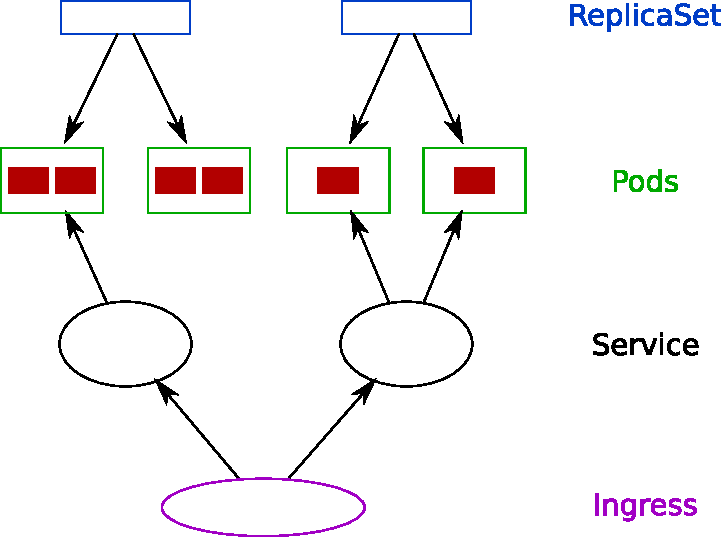
\includegraphics[width=0.8\textwidth]{img/arch-psir.pdf}
 \end{frame}
 
 \begin{frame}{Replica Sets}
  \begin{itemize}
   \item Defines replication of pods
   \item Will start/stop pods to match the wanted number of \texttt{replicates}
  \end{itemize}
 \end{frame}

 % Demo:
 % - start rs
 % - show it's running kubectl get pods/rs
 % - delete pod
 % - show it's replaced
 % - delete rs
 % - show it's gone
 
 \begin{frame}{Deployments}
  \centering
  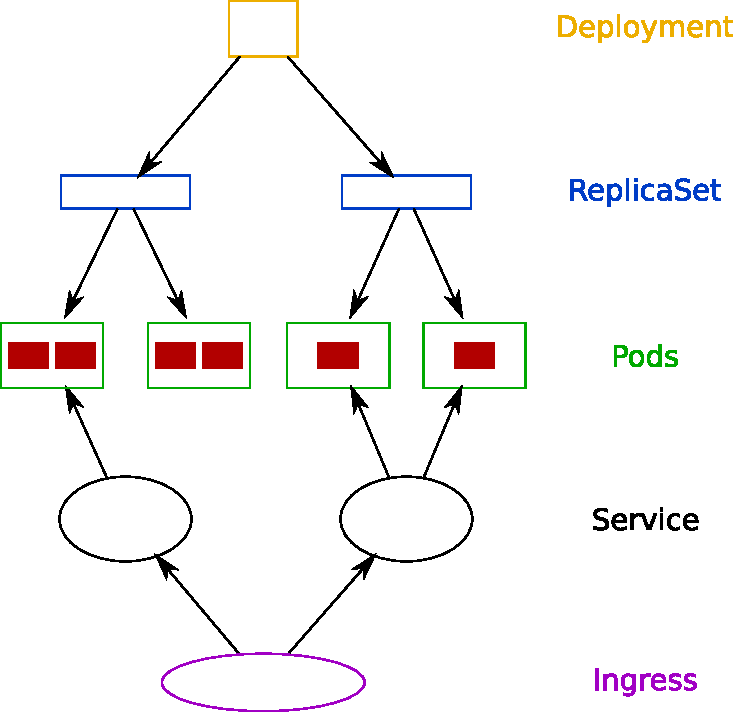
\includegraphics[width=0.8\textwidth]{img/arch-psird.pdf}
 \end{frame}

 \begin{frame}{Deployments}
  \begin{itemize}
   \item Deployments of replica sets
   \item Allows progressive deployment of new containers
  \end{itemize}
 \end{frame}
 
\begin{frame}
 \begin{columns}
  \column{0.35\textwidth}
   \begin{tikzpicture}
    \node[anchor=south west,inner sep=0] (image) at (0,0) {
\includegraphics[width=\textwidth]{img/creature.jpeg}};
    \framenode[3pt]{image} % opt. arg. is fade radius; mand. arg. is node name to frame
\end{tikzpicture}
  \column{0.65\textwidth}
  {\Large \bf Linus Östberg}
  
  {\small SciLifeLab Data Centre}

  \vspace{20pt}
  
  \begin{tabular}{cl}
   
\includegraphics[height=0.5cm]{img/github.pdf} & \href{https://github.com/talavis}{talavis} \\
   
\includegraphics[height=0.5cm]{img/slack.pdf} & \texttt{@lostb} \\
  \end{tabular}
 \end{columns}
 
 \vspace{50pt}
 
 \begin{columns}
 \column{0.55\textwidth}
 {\tiny \url{https://github.com/talavis/coffee-k8s}}
 \column{0.45\textwidth}
  
\includegraphics[height=0.8cm]{img/scilifelab-logo.pdf}
  \end{columns}
\end{frame}


\end{document}
